% =========================
% ANNEXE A — Questionnaire complet
% =========================
\Annexe{A}{Questionnaire complet}

\noindent Questionnaire (Google Form) : \url{https://docs.google.com/forms/d/1OhzCtKUQK7Z44ke8tMdHkosV9gpDlhxhAgjMddECBm8/edit}

\vspace{0.8cm}

% --- Deux screens côte à côte ---
\begin{figure}[H]
  \centering
  \begin{minipage}[t]{0.48\textwidth}
    \centering
    \includegraphics[width=\textwidth]{assets/17_annexe/Annexe_A_Screen1.png}
  \end{minipage}\hfill
  \begin{minipage}[t]{0.48\textwidth}
    \centering
    \includegraphics[width=\textwidth]{assets/17_annexe/Annexe_A_Screen2.png}
  \end{minipage}

  \vspace{0.4cm}
  \centering \textit{Extrait du formulaire Google Forms}
\end{figure}

\clearpage

% --- PDF complet du questionnaire ---
\includepdf[
  pages=-,
  scale=0.95,
  pagecommand={}
]{assets/17_annexe/Annexe_A_Questionnaire.pdf}

\clearpage


% =========================
% ANNEXE B — Résultats détaillés du questionnaire
% =========================
\Annexe{B}{Résultats détaillés du questionnaire}

\noindent Résultats (exports Google Forms) : graphiques + PDF récapitulatif.

\vspace{0.25cm}

% --- Page 1 : 2 graphiques (côte à côte) ---
\begin{figure}[H]
  \centering
  \begin{minipage}[t]{0.495\textwidth}
    \centering
    \includegraphics[width=\textwidth]{assets/17_annexe/Annexe_B_Graph_Reponses1.png}
  \end{minipage}\hfill
  \begin{minipage}[t]{0.495\textwidth}
    \centering
    \includegraphics[width=\textwidth]{assets/17_annexe/Annexe_B_Graph_Reponses2.png}
  \end{minipage}

  \vspace{-0.15cm}
  \caption*{\small\textit{Extraits 1 \& 2 — résultats du questionnaire (Google Forms)}}
\end{figure}

\clearpage

% --- Page 2 : 2 graphiques centrés ---
\vspace*{\fill}
\begin{figure}[H]
  \centering
  \begin{minipage}[t]{0.495\textwidth}
    \centering
    \includegraphics[width=\textwidth]{assets/17_annexe/Annexe_B_Graph_Reponses3.png}
  \end{minipage}\hfill
  \begin{minipage}[t]{0.495\textwidth}
    \centering
    \includegraphics[width=\textwidth]{assets/17_annexe/Annexe_B_Graph_Reponses4.png}
  \end{minipage}

  \vspace{-0.15cm}
  \caption*{\small\textit{Extraits 3 \& 4 — résultats du questionnaire (Google Forms)}}
\end{figure}
\vspace*{\fill}

\clearpage

% --- Page 3 : 2 graphiques centrés ---
\vspace*{\fill}
\begin{figure}[H]
  \centering
  \begin{minipage}[t]{0.495\textwidth}
    \centering
    \includegraphics[width=\textwidth]{assets/17_annexe/Annexe_B_Graph_Reponses5.png}
  \end{minipage}\hfill
  \begin{minipage}[t]{0.495\textwidth}
    \centering
    \includegraphics[width=\textwidth]{assets/17_annexe/Annexe_B_Graph_Reponses6.png}
  \end{minipage}

  \vspace{-0.15cm}
  \caption*{\small\textit{Extraits 5 \& 6 — résultats du questionnaire (Google Forms)}}
\end{figure}
\vspace*{\fill}

\clearpage

% --- PDF complet : 2 pages PDF sur 1 page A4 ---
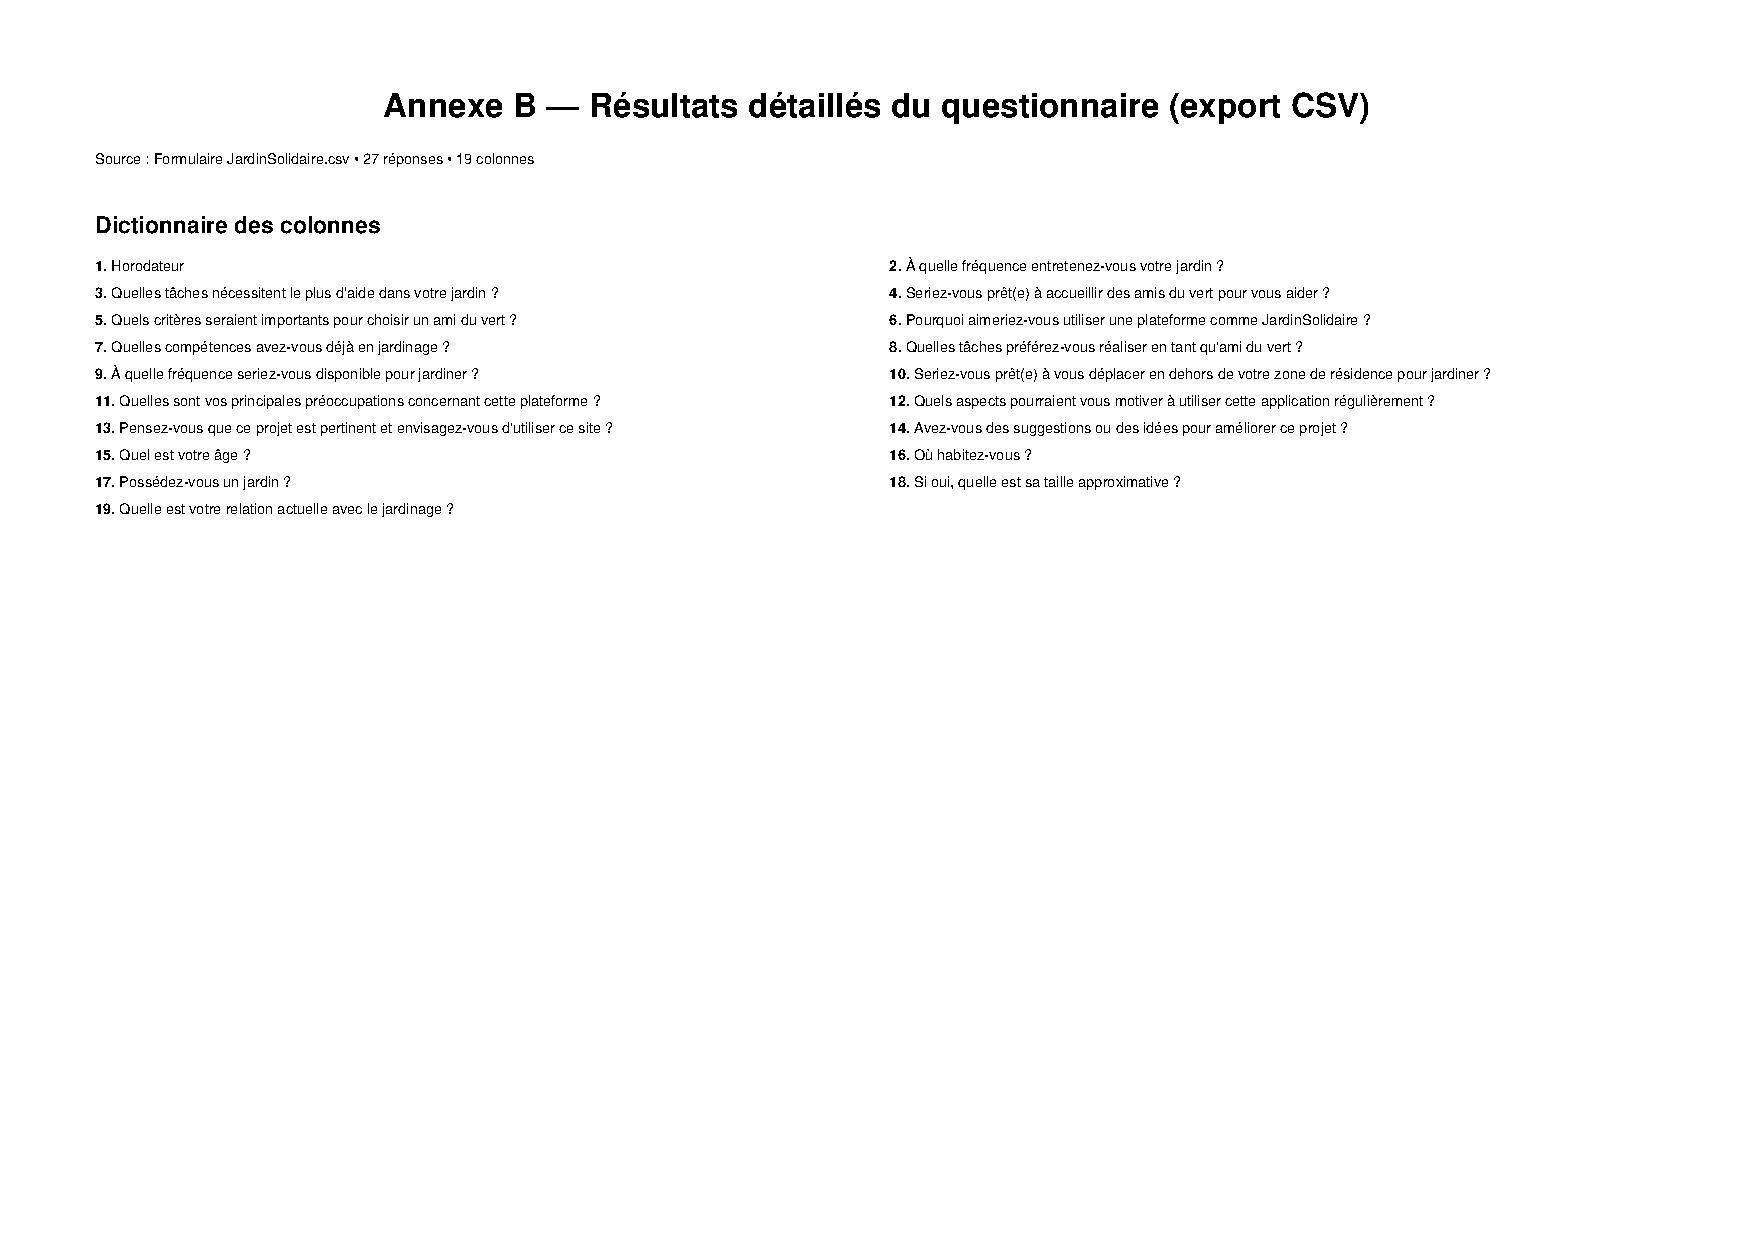
\includepdf[
  pages=-,
  nup=1x2,
  scale=0.92,
  delta=0 8pt,
  pagecommand={}
]{assets/17_annexe/Annexe_B_Resultats_questionnaire.pdf}

\clearpage

% =========================
% ANNEXE C — Cahier des charges
% =========================
\Annexe{C}{Cahier des charges}

\noindent Cahier des charges (document complet de la première version).


\begin{figure}[H]
  \centering
  \includegraphics[width=1.15\textwidth]{assets/17_annexe/Annexe_C_Cover_Cahier_des_Charges.png}
\end{figure}


% --- PDF complet : Cahier des charges ---
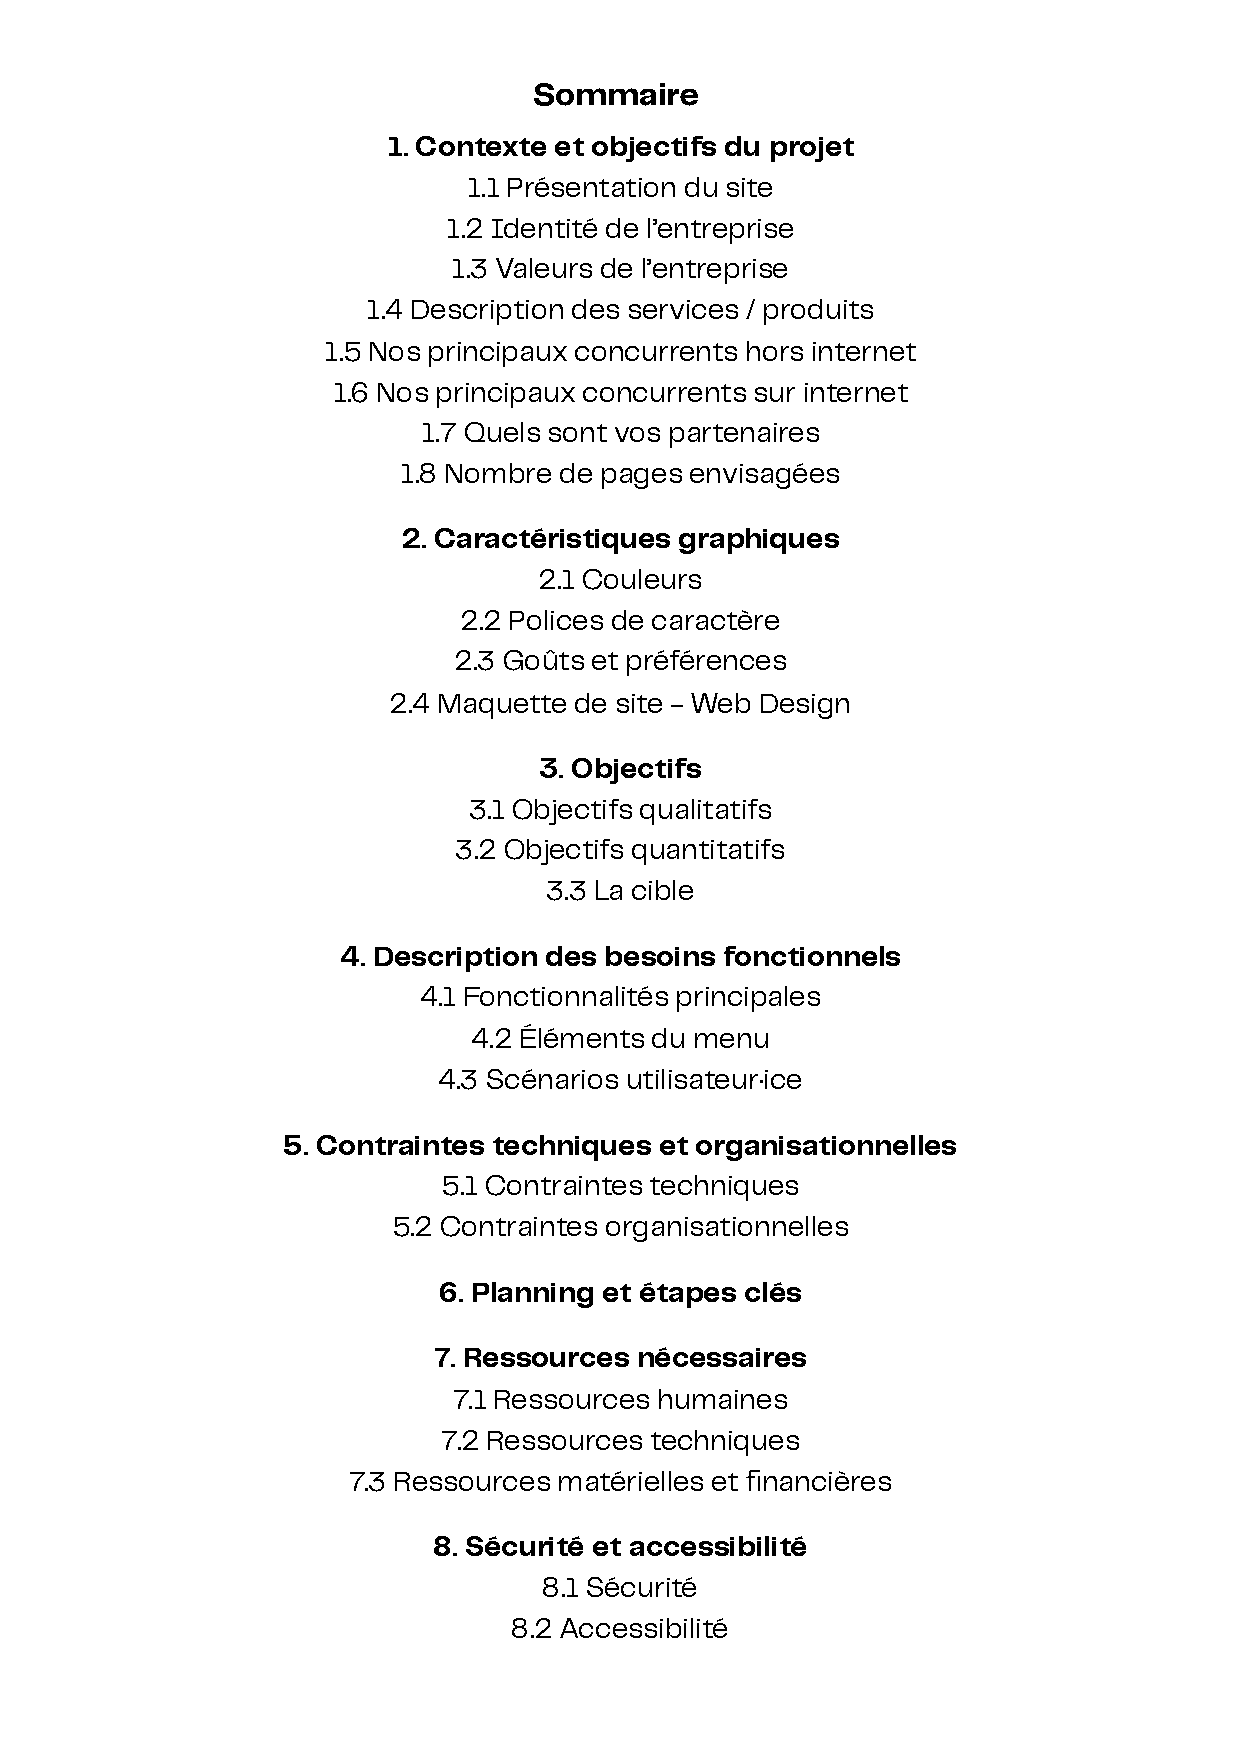
\includepdf[
  pages=-,
  scale=0.92,
  pagecommand={}
]{assets/17_annexe/Annexe_C_Cahier_des_Charges.pdf}

\clearpage
